
    \section{Quantum Complexity}
    \subsection{Quantum Mechanics}
    \setbeamercovered{invisible}
    \begin{frame}{Schrodinger's cat}
        \begin{columns}[onlytextwidth]
            \column{0.5\textwidth}
            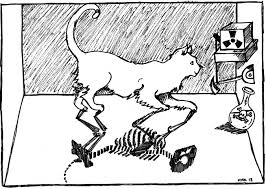
\includegraphics[width=\linewidth]{images/cat.jpg}
        \column{0.5\textwidth}
        \begin{itemize}
            \item Assume there is a cat in a box, with a handle 
            that will break the poison bottle based on the reaction of a quantum particle
            \pause
            \item Is the cat dead or alive?
            \pause
            \item Neither, the cat is bound to the \alert{SuperPosition} of the
            quantum particle, being both dead and alive at the same time.
        \end{itemize}
        
        \end{columns}
    \end{frame}
    \setbeamercovered{transparent}
    \begin{frame}{Why measurement alters the state}
        \begin{itemize}
            \item Niels Bohr  (Copenhagen interpretation):\\
            In essence this interpretation amounts to a sophisticated way of saying not to ask the question. Science relies on the notion of measurements and observations, so in essence asking in quantum mechanics “what is a measurement?” is equivalent to asking the axioms of euclidean geometry “what is a point?”.
        \end{itemize}
    \end{frame}
    \begin{frame}{Why measurement alters the state}
        \begin{itemize}
            \item Hugh Everett  (Many worlds interpretation):\\
            There is only one process in quantum mechanics, unitary evolution. What we perceive as measurements is just unitary evolution applied to the measuring equipment and the observer. Essentially the universe splits every time a measurement is performed, and one copy sees $|0\rangle$ while the other sees $|1\rangle$.            
        \end{itemize}
    \end{frame}
    \begin{frame}{Why measurement alters the state}
        \begin{itemize}
        
            \item David Bohm  (Non-local hidden variables):\\
            The third answer says that both of the previous answers are unacceptable, so quantum mechanics is somehow incomplete in the sense that there is an additional aspect that we’re missing. Non-local hidden variables is one proposal to fill that gap, but there are others.
        \end{itemize}
    \end{frame}
    \subsection{Quantum Computing}
    
    \begin{frame}{Qubits and data representation}
        \begin{itemize}
            \item We represent Superposition of data with a vector in complex space with a length of 1.
            \item We represent the value of the vector with the unit basis of our space.
            \item For the purpose of this lecture we follow the traditional representation by Qubits:
                \begin{itemize}
                    \item We represent one qubit with $|x\rangle $ with definition:\\
                    $|0\rangle := \begin{bmatrix}
                        1\\
                        0
                    \end{bmatrix}$
                    $|1\rangle := \begin{bmatrix}
                        0\\
                        1
                    \end{bmatrix}$
                    \item We define n not \alert{entangled} qubit with this notation:\\
                    $|x\rangle^{\oplus n} := \underbrace{|x\rangle|x\rangle \dots |x\rangle}_n $
                \end{itemize}
        \end{itemize}
    \end{frame}
    \begin{frame}{Qubits and data representation}
        \begin{itemize}
            \item Similarly we represent n \alert{entangled} multi-qubits with n basis vectors\\
            $|00\rangle := \begin{bmatrix}
                1\\
                0\\
                0\\
                0
            \end{bmatrix}$
            $|01\rangle := \begin{bmatrix}
                0\\
                1\\
                0\\
                0
            \end{bmatrix}$
            $|10\rangle := \begin{bmatrix}
                0\\
                0\\
                1\\
                0
            \end{bmatrix}$
            $|11\rangle := \begin{bmatrix}
                0\\
                0\\
                0\\
                1
            \end{bmatrix}$
        \end{itemize}
    \end{frame}

    \begin{frame}{Quantum Operations}
        Let us give an example of what a quantum operation looks like.
        We represent quantum operations by multiplying our data by an L2-norm preserving matrix e.g unitary matrices\\
        For example an elementary operation is controlled-NOT (CNOT) that is:\\
        \begin{center}
        $\begin{bmatrix}
            1&0&0&0\\
            0&1&0&0\\
            0&0&0&1\\
            0&0&1&0\\
        \end{bmatrix}$\\
    \end{center}
    it maps $|00\rangle \rightarrow |00\rangle$ , $|01\rangle \rightarrow |01\rangle$
    $|10\rangle \rightarrow |11\rangle$, $|11\rangle \rightarrow |10\rangle$. in other language
    it performs not on the second bit iff the first bit is true or it maps $|xy\rangle \rightarrow |x(x\oplus y)\rangle$

    \end{frame}
    
    % \begin{frame}[plain]{Plain frame}
    \begin{frame}{Measurement}
        We can measure our quantum state by projecting our quantum state vector onto 
        one of our \emph{Orthonormal Basis}. The probability of successful projection is equal to Coefficient power 2.
        for example in our data representation the matrix\\
        \begin{align*}
        \begin{bmatrix}
            \frac{1}{\sqrt{3}}\\
            \sqrt{\frac{2}{3}}
        \end{bmatrix}
        = \frac{1}{\sqrt{3}} |0\rangle + \sqrt{\frac{2}{3}} |1\rangle
    \end{align*}
    So when we measure we get $|0\rangle$ with the probability of 
    $\frac{1}{3}$ and we get $|1\rangle$ with probability of $\frac{2}{3}$.
    \end{frame}
    \begin{frame}{Measurement}
        \begin{block}{Quantum state}
            A quantum state is a n-dimensional complex vector with the length of 1. 
        \end{block}
        \pause
        \begin{block}{Quantum basis state}
            Quantum basis states are a collection of \textbf{Orthonormal basis}
            which we can measure our quantum state with them.
        \end{block}
        \pause
        \begin{block}{Measurement}
            Assume we have a multi-qubit like:\\
            $|a_1a_2 \dots a_n \rangle$ where 
            $\sum_{n = 1}^{n} a_i^2 = 1$
            we can measure this qubit in basis states where the probability
            of us measuring this qubit onto $ith$ state is $a_i^2$
        \end{block}
    \end{frame}
    \begin{frame}{Measurement}
        \begin{exampleblock}{example}
            Assume we can perform a quantum operation which rotates our quantum state
            by $45^o$ the matrix resembling this operation is as follows
            $ \frac{1}{\sqrt{2}}
            \begin{bmatrix}
                1&1\\
                -1&1
            \end{bmatrix}$
            performing this operation twice is equivalent to the NOT operation:\\
            \begin{align*}
                |x\rangle \rightarrow 
                \frac{1}{\sqrt{2}}
                    \begin{bmatrix}
                        1\\
                        -1
                    \end{bmatrix}
                    \rightarrow |1\rangle,
                |1\rangle \rightarrow 
                \frac{1}{\sqrt{2}}
                    \begin{bmatrix}
                        1\\
                        1
                    \end{bmatrix}
                    \rightarrow |0\rangle
            \end{align*}
            but if we perform this operation once then measure and perform it again we get $|0\rangle$ or $|1\rangle$
            
        \end{exampleblock}
    \end{frame}
    \begin{frame}{Entanglement}
        Assume we have a 2-qubit :
        $$\alpha |00\rangle + \beta |01\rangle + \gamma |10\rangle + \delta |11\rangle$$
        we can perform an operation only on the second qubit by finding the tensor product of our transformation:
        $$
        \frac{1}{\sqrt{2}}
            \begin{bmatrix}
                1&-1\\
                1&1
            \end{bmatrix}
            \otimes \begin{bmatrix}
                1&0\\
                0&1
            \end{bmatrix}
            = \frac{1}{\sqrt{2}}
            \begin{bmatrix}
                1&-1&0&0\\
                1&1&0&0\\
                0&0&1&-1\\
                0&0&1&1
            \end{bmatrix}
        $$
    \end{frame}
    \begin{frame}{Entanglement}
        the probability of us measuring the first qubit $|0\rangle$ is equal to 
        $\alpha^2 + \beta^2$. Assuming we measured the first one $|0\rangle$ the state of the second qubit collapses to:
        $$\frac
        {\alpha |0\rangle + \beta |1\rangle}
        {\sqrt{\alpha^2 + \beta^2}}$$
    \end{frame}
    \begin{frame}{Entanglement}
        \begin{block}{Proof}
            \begin{gather}
                x_2 = \alpha' |0\rangle + \beta' |1\rangle\\
                \beta'^2 = P(x_2 = |1\rangle | x_1 = |0\rangle)=
                \frac
                {P(x_2 = |1\rangle \land x_1 = |0\rangle)}
                {P(x_1 = |0\rangle)}
                = \frac{\beta^2}{\alpha^2 + \beta^2} \\
                \alpha'^2 = P(x_2 = |0\rangle | x_1 = |0\rangle) =
                \frac
                {P(x_2 = |0\rangle \land x_1 = |0\rangle)}
                {P(x_1 = |0\rangle)}
                = \frac{\alpha^2}{\alpha^2 + \beta^2}
            \end{gather}
        \end{block}
    \end{frame}
    \begin{frame}{Bell's inequality}
        \begin{itemize}
            \item<1-> In 1935, Einstein, Podolsky and Rosen wrote a famous paper where they brought to widespread
            attention the tension between quantum mechanics and relativity. One thing that relativity says
            is that you can’t send information faster than light.
            \item<2-> In 1964 Bell played the roll of a quantum complexity theorist. He said, let’s compare entangle­ ment against classical correlation as resources to perform some task.
        \end{itemize}
        \begin{center}
            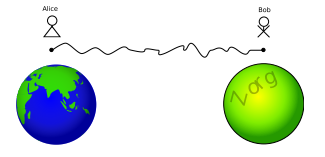
\includegraphics[scale=0.5]{images/ent.png}
        \end{center}
        
    \end{frame}
    \begin{frame}{Quantum Circuits}
        We present a series of quantum operations on qubits via a circuit which 
        each operation represents itself as a gate in our circuit
        \begin{block}{CNOT gate}
            \begin{center}
            \begin{quantikz}
                \lstick{x} & \ctrl{1} &
                \wire[l][1]["x"{above,pos=0.2}]{a} \\
                \lstick{y} & \targ{} & \rstick{x+y}
                \end{quantikz}
            \end{center}
        \end{block}
    \end{frame}
    \begin{frame}{Quantum Circuits}
        \begin{block}{Hadamard Gate}
            Hadarmand gate switches between $|0\rangle,|1\rangle$ and
            $|0\rangle+|1\rangle,|0\rangle-|1\rangle$ basis. The matrix for this operation
            is as follows: $
            \begin{bmatrix}
                \frac{1}{\sqrt{2}}&\frac{1}{\sqrt{2}}\\
                \frac{1}{\sqrt{2}}&-\frac{1}{\sqrt{2}}
            \end{bmatrix}$
            We represent this operation by following gate:\\
            \begin{center}
            \begin{quantikz}
                && \gate{H} &&
            \end{quantikz}
        \end{center}
            
        \end{block}
    \end{frame}
    \begin{frame}{Quantum Circuits}
        \begin{block}{Tofoli's Gate (CCNOT)}
            $$\begin{bmatrix}
                1&0&0&0&0&0&0&0\\
                0&1&0&0&0&0&0&0\\
                0&0&1&0&0&0&0&0\\
                0&0&0&1&0&0&0&0\\
                0&0&0&0&1&0&0&0\\
                0&0&0&0&0&1&0&0\\
                0&0&0&0&0&0&0&1\\
                0&0&0&0&0&0&1&0\\
            \end{bmatrix}$$
            $$
            (a,b,c) \rightarrow (a,b,c \oplus (a \land b))
            $$
        \end{block}
    \end{frame}
    \begin{frame}{Quantum Circuits}
        \begin{exampleblock}{Circuit example 1 }
            From what we learned we can introduce a circuit starting from unentangled states creating 
            entangled states\footnote{\url{https://en.wikipedia.org/wiki/Bell_state}}.\\
            \begin{center}
            \begin{quantikz}
                \lstick{\ket{0}} & \gate{H} & \ctrl{1} &&\\
                \lstick{\ket{0}} && \targ{} &&& \rstick{\ket{00} + \ket{11}}
            \end{quantikz}
        \end{center}
        \end{exampleblock}
    \end{frame}
    \begin{frame}{Quantum Circuits}
        \begin{exampleblock}{Circuit example 2 }
            The example from before about measurement between computations is as follows:\\
            \begin{center}
                \begin{quantikz}
                    \lstick{\ket{q}} & \gate{H} & \gate{H} & \meter{} & \rstick{NOT \ket{q}}\\
                    \lstick{\ket{q}} & \gate{H} & \meter{} & \gate{H} & \meter{} & \rstick{\ket{q} or NOT \ket{q}}
                \end{quantikz}
                % \begin{quantikz}
                %     \lstick{\ket{q}} & \gate{H} & \gate{H} & \meter{} & \rstick{NOT \ket{q}}
                    
                % \end{quantikz}
                
            \end{center}
        \end{exampleblock}
    \end{frame}
    \begin{frame}{Quantum Computation}
        \begin{itemize}
            \item What is the quantum computation model?
            \pause
            \item This question was answered in rigorous terms by Bernstein and Vzirani in a 70 page paper in 1993
            who defined a quantum Turing machine that could have the tape head and symbols and superpositions.
            \pause
            \item Independently, Andy Yao defined quantum circuits, which are computationally equivalent. This is
            what people use today because they are simpler.
        \end{itemize}
    \end{frame}
    \subsection {Quantum Complexity}
    % \begin{frame}[t]
    \begin{frame}{Reminder}
        \begin{block}{P}
            P is the class of languages $L \subset \{0,1\}^*$ for which there exists a Turing machine M and a polynomial q
            so that for inputs $x \in \{0,1\}^n$, M Terminates in at most $q(n)$ steps and accepts iff $x \in L$
        \end{block}
        \pause
        \begin{block}{PSPACE}
            PSPACE is defined like P except we're limited by $q(n)$ steps, rather than time.
        \end{block}
        \pause
        \begin{block}{EXP}
            EXP is defined like P, but we're limited by $2^{q(n)}$ steps.
        \end{block}
        
    \end{frame}
    \begin{frame}{Reminder}
        \begin{block}{BPP}
            P is the class of languages $L \subset \{0,1\}^*$ for which there exists a Turing machine \textbf{probabilistic} M and a polynomial q
            so that for inputs $x \in \{0,1\}^n$, M Terminates in at most $q(n)$ steps and
            \begin{itemize}
                \item if $x \in L$, then M accepts with probability $> \sfrac{2}{3}$
                \item if $x \notin L$, then M accepts with probability $< \sfrac{1}{3}$
            \end{itemize}
            Or equivalently there exists a Turing machine M with two inputs x,r both in $\{0,1\}^n$
            which
            \begin{itemize}
                \item if $x \in L$, then M(x,r) accepts for at least $\sfrac{2}{3}$ values of r.
                \item if $x \notin L$, then M(x,r) accept for at most $\sfrac{1}{3}$ values of r.
            \end{itemize}
            \pause
            \begin{alertblock}{constants importance}
                the constants are not important; we can amplify the success probability as much as we want by chaining Turing machines.
            \end{alertblock}
        \end{block}
    \end{frame}
    \begin{frame}{BQP}
        \begin{block}{Definition}
            BQP is the class of languages  $L \subset \{0,1\}^*$ for which there exists a \emph{uniform}
            family of polynomial-size quantum circuit $\{C_n\}$ over some basis of universal gates and a polynomial q
            so that for all n and inputs $x \in \{0,1\}^n$.
            \begin{itemize}
                \item if $x \in L$, then $C_n(|x\rangle|0\rangle^{\otimes q(n)})$ accepts with probability $> \sfrac{2}{3}$
                \item if $x \notin L$, then $C_n(|x\rangle|0\rangle^{\otimes q(n)})$ accepts with probability $< \sfrac{1}{3}$
            \end{itemize}
        \end{block}
        \pause
        \begin{alertblock}{Difference with BPP}
            Unlike BPP we cannot extract the element of randomness out of our definition of a quantum circuit.
            This is the fundamental difference of quantum complexity classes and traditional ones. 
        \end{alertblock}
    \end{frame}
    \setbeamercovered{invisible}
    \begin{frame}{BQP properties}
        \begin{block}{$P \subset BPP$}
            \pause
            Just don't use randomness
        \end{block}
        \pause
        \begin{block}{$BPP \subset PSPACE$}
            \pause
            Run the problem for each possible r and keep count of how many are accepted.
        \end{block}
        \pause
        \begin{block}{$PSPACE \subset EXP$}
            \pause
            Polynomial space can go through exponentially many configurations without looping.
        \end{block}
    \end{frame}
    \begin{frame}{Universal Quantum gates}
        \begin{block}{Solovay-Kitaev Theorem}
            With a finite set of gates, we can approximate any n-qubit unitary within L2 accuracy $\epsilon$
            using $2^n(n+polylog(\sfrac{1}{\epsilon}))$ gates.
            % (For example, Hadamard and Toffoli gates). In fact, with CNOT and
            % arbitrary 1-qubit gates, we can apply any n-qubit unitary.
        \end{block}
        \pause
        \begin{block}{$SU(2)$}
            $$SU(2) := \begin{bmatrix}
                \alpha & -\bar{\beta} \\
                \beta & \bar{\alpha}
            \end{bmatrix}
            : \alpha, \beta \in \mathbb{C}, |\alpha|^2 + |\beta|^2 = 1$$
        \end{block}
        \begin{block}{Universal Quantum gates}
            A set of \textbf{universal quantum gates} is any set of gates to which any operation possible on a quantum computer can be reduced, that is, any other unitary operation can be expressed as a finite sequence of gates from the set. 
        \end{block}
    \end{frame}
    \begin{frame}{Universal Quantum Gates}
        \begin{exampleblock}{Some examples of Universal Quantum Gate}
            \begin{itemize}
                \item Rotational operators $R_x(\theta),R_y(\theta),R_z(\theta)$
                and phase shift operator $P(\phi)$ and CNOT can be used to form several Universal gate set
                \item Tofoli(CCNOT) + Hadamard gate. 
                The Toffoli gate alone forms a set of universal gates for 
                reversible Boolean algebraic logic circuits, which encompass all 
                classical computation.
            \end{itemize}
        \end{exampleblock}
    \end{frame}
    \begin{frame}{Universal Quantum Gates}
        \begin{block}{formalized Solovay-Kitaev Theorem}
            Let $\mathcal{G}$ be a finite set of elements in SU(2) containing its own inverses (so 
    ($g \in \mathcal{G}$ implies $g^{-1} \in \mathcal{G}$)
        and such that the group $\langle \mathcal{G} \rangle$ they generate is dense in SU(2). Consider some 
    $\epsilon > 0$. Then there is a constant $c$ such that for any 
        $U \in SU(2)$, there is a sequence $S$ of gates from $\mathcal {G}$ of length 
    $O(log^c(\sfrac{1}{\epsilon}))$ such that $||S-U|| \leq \epsilon$. That is, 
S approximates U to operator norm error.
        \end{block}
    \end{frame}
    \begin{frame}{BQP Properties Continued}
        \begin{block}{$P \subseteq BQP$}
            \pause
            Any classical circuit can be simulated by a quantum circuit. (for more information see chapter 3.1.2 of \cite{Nielsen11})
        \end{block}
        \begin{block}{$BPP \subseteq BQP$}
            \pause
            We can generate a random number as much as we want, for example using Hadamard gate and 
            $|0\rangle$ gives us a random bit. \footnote{Well not exactly, see https://people.eecs.berkeley.edu/~vazirani/f04quantum/notes/lec5/lec5.pdf}

        \end{block}
        \begin{block}{$BQP \subseteq EXP$}
            \pause
            Since a quantum state can be written as $|\psi \rangle = \sum a_x |x\rangle$, we can simulate
            the whole evolution of quantum vectors with classical computers, within exponential time at most. \footnote{we use BQP-completness of APPROX-QCIRCUIT-PROB}
        \end{block}
    \end{frame}
    \begin{frame}{BQP Properties Continued}
        \begin{block}{$BQP \subseteq PSPACE$}
            by using Feynmann's path integral we can simulate the circuit in polynomial time.
            Schrodinger's picture: 
            $$P(x_m) = |\langle x_m | U_m U_{m-1} \dots U_1| 0 \rangle|^2$$
            While in Feynman's path algorithm $P(x_m)$ is calculated by summing up the contributions of $(2^n)^{m-1}$:
            $$P(x_m) = |\langle x_m | U | 0 \rangle ^n|^2 = 
            | \sum_{x_1,x_2 \dots x_{m-1} \in \{0,1\}^n }^{} \prod_{j=1}^{m} \langle x_j | U_j | x_{j-1} \rangle |^2 $$
            Schrodinger's take $ ~ m 2^n$ time and $2^n$ space while Feynman's take 
            $~ 4^m$ time and $~ m + n$ space.
        \end{block}
    \end{frame}
    \begin{frame}{BQP Properties Continued}
        \begin{block}{$P^P = P^{\#P}$}
            
        \end{block}
        \pause
        \begin{block}{$BQP \subseteq P^{\# P} \subseteq PSPACE$}
            Since we can do counting in polynomial space, $P^{\#P} \subseteq PSPACE$. Also $\# P$ can follow all paths 
            nondeterministic in Feynman's path integral
        \end{block}
        \pause
        \begin{block}{$BQP \subseteq PP$}
            
        \end{block}
    \end{frame}
    \begin{frame}{BQP Properties Continued}
        \begin{block}{Quantum Complexity Inclusion}
            $$P \subseteq BPP \subseteq BQP \subseteq PP \subseteq P^{\# P} \subseteq PSPACE \subseteq EXP$$
        \end{block}
        \begin{center}
            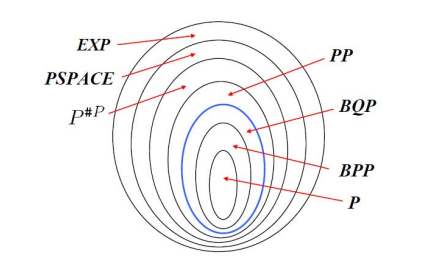
\includegraphics[scale = 0.5]{images/Complexdiag.png}
        \end{center}
    \end{frame}
    \setbeamercovered{transparent}
    \begin{frame}{Some more}
        \begin{block}{$BPP \neq BQP$ ?}
            Can we prove that quantum computer exceeds classical computers? The answer is no since it would imply
            $P \neq PSPACE$ which is as difficult to prove as $P \neq NP$
        \end{block}
        \pause
        \begin{block}{Where is NP?}
            We don't know!. The conjecture is that $NP \nsubseteq BQP$ which means quantum computer cannot solve NP-complete
            problems in polynomial time. However we have no idea whether $BQP \nsubseteq NP$ or not.
        \end{block}
        \pause
        \begin{block}{$BQP^{BQP} = BQP$}
            We use uncomputing.
        \end{block}
    \end{frame}
    \subsection{Quantum Query model}
    \begin{frame}{Quantum Query model}
        We have already discussed how proving complexity lower bounds on quantum 
        computation seems very difficult. Just as with classical complexity, then, we turn to simplified, 
        idealized models of computation in the hopes of proving something and gaining intuitions. 
        We try to model, in the quantum world, the classical idea of a \'bounded-query\' algorithm, 
        one which has access to a very large (binary) input and tries to compute some predicate of the input 
        without looking at too many input bits. We think of this input as a function $f(x): \{0,1\}^n \rightarrow \{0,1\}$.
    \end{frame}
    \begin{frame}{Quantum Query model}
        These query unitaries are usually restricted into two types:
        \begin{block}{controlled-not query}
            maps basis state $|x,w\rangle$ to $|x,w \oplus f(x) \rangle$
        \end{block}
        \begin{block}{textitphase query}
            maps $|x\rangle$ to $(-1)^{f(x)}|x\rangle$
        \end{block}
        \begin{block}{Equivalency}
            These two models are equivalent.
        \end{block}
    \end{frame}
    \begin{frame}{Deutch-Joza Algorithm}
        The function takes n-bit binary values as input and produces either 
        a 0 or a 1 as output for each such value. We are \textbf{promised} that the function 
        is either constant (0 on all inputs or 1 on all inputs) 
        or balanced (1 for exactly half of the input domain and 0 for the other half).\\
        The task is to find whether the oracle is constant or balanced.
        \begin{block}{Classical approach}
            In classical approach for n-bits input we need $2^{n-1} + 1$ queries to get the answer.
            We have to at least check half of the possible outcomes.
        \end{block}
    \end{frame}
    \begin{frame}{Deutch-Joza Algorithm }
        \begin{center}
            \begin{quantikz}
                \lstick{$|0\rangle^{\otimes n}$}&\gate{H}&\gate[2][1.7cm]{U}\gateinput{$x$}\gateoutput{$x$} & \gate{H} & \meter{} & \\
                \lstick{\ket{1}} & \gate{H} & \gateinput{$y$}\gateoutput{$y\oplus f(x)$} &
            \end{quantikz}
        \end{center}
        The algorithm starts with $n+1$ bit state $|0\rangle^{\oplus n} |1\rangle$, after Hadamard's transform we obtain:
        $$\frac{1}{\sqrt{2^{n+1}}} \sum_{x=0}^{2^n-1} |x\rangle(|0\rangle - |1\rangle)$$
    \end{frame}
    \begin{frame}{Deutch-Joza Algorithm }
        applying the query gives us:
        $$\frac{1}{\sqrt{2^{n+1}}} \sum_{x=0}^{2^n-1} (-1)^{f(x)}|x\rangle(|0\rangle - |1\rangle)$$
        let's forget about last bit so we have:
        $$\frac{1}{\sqrt{2^{n+1}}} \sum_{x=0}^{2^n-1} (-1)^{f(x)}|x\rangle$$
        we also know that:
        $$ H^{\oplus n}|k\rangle = \frac{1}{\sqrt{2^n}} \sum_{j=0}^{2^n-1} (-1)^{k.j} |j\rangle$$
        where $j.k = j_0 . k_0 \oplus j_1 . k_1 \oplus \dots j_{n-1} . k_{n-1}$ where $\oplus$ is addition module 2.
    \end{frame}
    \begin{frame}{Deutch-Joza Algorithm}
        \begin{block}{Proof}
            n=1: $$|x\rangle = \begin{bmatrix}
                \alpha \\
                \beta
            \end{bmatrix} = \alpha |0\rangle + \beta |1\rangle$$
            $$H |x\rangle = \frac{1}{\sqrt{2}} \begin{bmatrix}
                \alpha + \beta \\
                \alpha - \beta
            \end{bmatrix} = \frac{1}{\sqrt{2}} (\alpha + \beta) |0\rangle + (\alpha - \beta) |1\rangle$$
            $$H |x\rangle = \frac{1}{\sqrt{2}} ((-1)^{x.0} |0\rangle + (-1)^{x.1} |1 \rangle)$$
            $$H |x\rangle = \frac{1}{\sqrt{2}} \sum_{j=0}^{1} (-1)^{xj} |j\rangle$$

        \end{block}
    \end{frame}
    \begin{frame}{Deutch-Joza Algorithm}
        \begin{block}{Proof}
            $$H^{\otimes n} |x_1,x_2\dots x_n \rangle = \sum_{j_1,j_2 \dots j_n \in \{0,1\} } \frac{(-1)^{(x_1j_1 + x_2j_2 + \dots x_nj_n)} |j_1,j_2 \dots j_n \rangle}{\sqrt{2^n}}$$
    
        \end{block}
        Therefor applying Hadamard gate the second time gives us
        $$\frac{1}{\sqrt{2^n}} \sum_{x=0}^{2^n-1} (-1)^{f(x)} \left[ \frac{1}{\sqrt{2^n}} \sum_{y=0}^{2^n-1} (-1)^{x.y} |y\rangle \right] $$
        $$\sum_{y=0}^{2^n-1} \left[ \frac{1}{2^n} \sum_{x=0}^{2^n-1} (-1)^{f(x)} (-1)^{x.y} \right] |y\rangle $$
    \end{frame}
    \begin{frame}{Deutch-Joza Algorithm}
        So the probability of state $|0\rangle$ to be measured is
        $$| \frac{1}{2^n} \sum_{x=0}^{2^n-1} (-1)^{f(x)} |^2$$
        this evaluates to 1 if $f$ is constant and 0 if $f$ is balanced.
        in the other words the end measurement will be $|0\rangle^{\otimes n}$ iff $f(x)$ is constant.
    \end{frame}
    \begin{frame}{Bernstein-Vazarani Algorithm}
        Suppose that there is a Boolean function, $f : \{0,1\}^n \rightarrow \{0,1\}$. The \textbf{promise} is that,
        the $f$ is in form of $s.x$ which is inner product of $s$ and $x$ module 2.
        \begin{block}{Classical approach}
            We can query basis strings and find the secret:
            $$f(100\dots0) = s_1$$
            $$f(010\dots0) = s_2$$
            $$\dots$$
            $$f(000\dots1) = s_n$$
        \end{block}
    \end{frame}
    \begin{frame}{Bernstein-Vazarani Algorithm}
        \begin{center}
        \begin{quantikz}
            \lstick{\ket{0}} & \gate{H} & \gate[5]{f} & \gate{H} & \rstick{$|s_1\rangle$}\\
            \lstick{\ket{0}} & \gate{H} &  & \gate{H} & \rstick{$|s_2\rangle$}\\
            \lstick{\ket{0}} & \gate{H} &  & \gate{H} & \rstick{$|s_3\rangle$}\\
            \setwiretype{n} \lstick{$\dots$} & \midstick{$\dots$} &  & \midstick{$\dots$} & \rstick{$\dots$}\\
            \lstick{\ket{0}} & \gate{H} &  & \gate{H} & \rstick{$|s_n\rangle$}\\
        \end{quantikz}
    \end{center}
    \end{frame}
    \begin{frame}{Bernstein-Vazarani Algorithm}
        \begin{center}
        \begin{gather}
            |0\rangle^{\otimes n} \rightarrow \frac{1}{2^n} \sum_{x\in\{0,1\}^n |x\rangle}\\
            \rightarrow \frac{1}{2^n} \sum_{x\in\{0,1\}^n (-1)^{f(x)} |x\rangle}\\
            = \frac{1}{2^n} \sum_{x\in\{0,1\}^n (-1)^{s.x} |x\rangle} \\
            = \frac{1}{2^n} \sum_{x\in\{0,1\}^n} (-1)^{s_1x_1} \dots (-1)^{s_nx_n}  |x\rangle
        \end{gather}
    \end{center}
    \end{frame}
    % \begin{frame}[noframenumbering]{No frame numbering}
    % \begin{frame}{No frame numbering}
    %     This frame is not numbered and is citing reference \cite{knuth74}.
    % \end{frame}
    
    % \begin{frame}{Typesetting and Math}
    %     The packages \texttt{fontenc} and \texttt{FiraSans}\footnote{\url{https://fonts.google.com/specimen/Fira+Sans}}\textsuperscript{,}\footnote{\url{http://mozilla.github.io/Fira/}} are used to properly set the main fonts.
    %     \vfill
    %     This theme provides styling commands to typeset \emph{emphasized}, \alert{alerted}, \textbf{bold}, \textcolor{example}{example text}, \dots
    %     \vfill
    %     \texttt{FiraSans} also provides support for mathematical symbols:
    %     \begin{align*}
    %         e^{i\pi} + 1 & = 0, \\
    %         \int_{-\infty}^\infty e^{-x^2}\,\mathrm{d}x & = \sqrt{\pi}.
    %     \end{align*}
    % \end{frame}
    % \section{new section}
    % \begin{frame}

    % \end{frame}
    % \begin{frame}

    % \end{frame}
    % \begin{frame}

    % \end{frame}